\documentclass[]{article}
\usepackage{lmodern}
\usepackage{amssymb,amsmath}
\usepackage{ifxetex,ifluatex}
\usepackage{fixltx2e} % provides \textsubscript

\ifnum 0\ifxetex 1\fi\ifluatex 1\fi=0 % if pdftex
  \usepackage[T1]{fontenc}
  \usepackage[utf8]{inputenc}
  \usepackage[french]{babel}
\else % if luatex or xelatex
  \ifxetex
    \usepackage{mathspec}
  \else
    \usepackage{fontspec}
  \fi
  \defaultfontfeatures{Ligatures=TeX,Scale=MatchLowercase}
\fi
% use upquote if available, for straight quotes in verbatim environments
\IfFileExists{upquote.sty}{\usepackage{upquote}}{}
% use microtype if available
\IfFileExists{microtype.sty}{%
\usepackage[]{microtype}
\UseMicrotypeSet[protrusion]{basicmath} % disable protrusion for tt fonts
}{}
\PassOptionsToPackage{hyphens}{url} % url is loaded by hyperref
\usepackage[unicode=true]{hyperref}
\hypersetup{
            pdfborder={0 0 0},
            breaklinks=true}
\urlstyle{same}  % don't use monospace font for urls
\usepackage{graphicx,grffile}
\makeatletter
\def\maxwidth{\ifdim\Gin@nat@width>\linewidth\linewidth\else\Gin@nat@width\fi}
\def\maxheight{\ifdim\Gin@nat@height>\textheight\textheight\else\Gin@nat@height\fi}
\makeatother
% Scale images if necessary, so that they will not overflow the page
% margins by default, and it is still possible to overwrite the defaults
% using explicit options in \includegraphics[width, height, ...]{}
\setkeys{Gin}{width=\maxwidth,height=\maxheight,keepaspectratio}
\IfFileExists{parskip.sty}{%
\usepackage{parskip}
}{% else
\setlength{\parindent}{0pt}
\setlength{\parskip}{6pt plus 2pt minus 1pt}
}
\setlength{\emergencystretch}{3em}  % prevent overfull lines
\providecommand{\tightlist}{%
  \setlength{\itemsep}{0pt}\setlength{\parskip}{0pt}}
%\setcounter{secnumdepth}{0}
% Redefines (sub)paragraphs to behave more like sections
\ifx\paragraph\undefined\else
\let\oldparagraph\paragraph
\renewcommand{\paragraph}[1]{\oldparagraph{#1}\mbox{}}
\fi
\ifx\subparagraph\undefined\else
\let\oldsubparagraph\subparagraph
\renewcommand{\subparagraph}[1]{\oldsubparagraph{#1}\mbox{}}
\fi

% set default figure placement to htbp
\makeatletter
\def\fps@figure{htbp}
\makeatother
\usepackage{hyperref}
\usepackage{array}
\date{}
\usepackage[margin=3.5cm]{geometry}
%En-tête et pied de page
\usepackage{fancyhdr}
\usepackage{tgadventor}
\pagestyle{fancy}
%En-tête
\fancyhead[L]{\leftmark}
\fancyhead[R]{}
%Pied de page
\fancyfoot[C]{\thepage}

\setcounter{tocdepth}{2} 
\begin{document}


\makeatletter
\begin{titlepage}
\centering
\textsc{Maud LAURENT - Valentin NORBERTO - Valentin PEYREGNE} \\
Tuteurs : Cyril MARCH - Guillaume PENAUD \\
\vspace{1cm}
\textsc{\today}\\
\vspace{5cm}

\includegraphics[width=0.25\textwidth]{Images/download.jpeg} \\
\vspace{1cm}
\Huge{Projet tuteuré \\ Déploiement et provisionnement d’un IAAS avec Openstack et Terraform}\\
\vfill
\end{titlepage}
\makeatother

\tableofcontents
\newpage

\section{Introduction}\label{introduction}

\subsection{Infrastructure as code}\label{infrastructure-as-code}

L'infrastructure as code ou encore \og infrastructure programmable \fg est
une technique qui vise à administrer une infrastructure via du code (avec divers langages possibles suivant la technologie utilisée).

L'IAC est utilisée à la fois pour gérer des configurations, mais aussi pour déployer et automatiser le
provisionnement d'une infrastructure. L'entreprise possède donc le code
pour pouvoir fournir et gérer nos serveurs tout en permettant
d'automatiser les tâches.

L'IAC, n'est plus seulement utilisée par les administrateurs systèmes. En effet les développeurs de logiciels et d'applications
peuvent facilement écrire un code d'infrastructure pour pouvoir se créer
un environnement à des fins expérimentales pour tester leurs logiciels.

De nombreux outils propose un système d'infrastructure as code. Par exemple Vagrant va permettre de créer un environnement virtuel grâce au code contenu dans
le Vagrantfile, ou encore Ansible qui va permettre l'installation de logiciels sur une instance. \\
Plus récemment, le logiciel Docker permet
d'automatiser le déploiement d'applications dans des conteneurs
logiciels. Il utilise également l'IAC avec les dockerfile. 

L'IAC permet de suivre les modifications d'une
infrastructure, en cas de problème, il sera alors très simple de revenir
à la configuration précédente. 

Cependant, l'infrastructure as code possède aussi des inconvénients. Une mauvaise configuration sera dupliquée sur toutes les machines concernées.
Il faut aussi faire attention aux modifications des machines pour éviter un éventuel problème de configuration au seins de l'infrastructure.

\subsection{Mouvance du Devops}\label{mouvance-devops}

Devops est la concaténation du mot anglais \emph{development} et
\emph{operations}. Au début de l'informatique en
entreprise, les applications ne jouaient pas un grand rôle et étaient
peu intégrées, il n'y avait alors pas de séparation entre développement
et opérations, la même équipe d'informaticiens se chargeait à la fois du
développement de l'application et de sa maintenance.

L'évolution de l'informatique d'entreprise a entraîné l'évolution de
l'utilisation des logiciels. Aujourd'hui, les logiciels ont une place
beaucoup plus importante ce qui a conduit à une
séparation du développement et de la partie opérationnelle en deux
équipes distinctes. L'équipe de développement apportait les changements
aux logiciels souvent le plus rapidement possible pour un moindre coût
tandis que l'équipe opération garantissait la stabilité du système en se
concentrant sur la qualité. 

L'objectif du mouvement devops est de cordonner l'ensemble des équipes du système d'information.

\subsection{Le cloud computing}\label{le-cloud-computing}

Le Cloud computing est un concept qui va permettre d'utiliser des
ressources informatiques sans les posséder réellement, de fournir des
services ou des applications accessibles partout depuis internet. Il y a
de nombreux avantages à utiliser un cloud computing. 

Tout d'abord, l'utilisateur n'a pas d'infrastructure à gérer, ce qui est parfois plus
simple pour des entreprises, car c'est le fournisseur cloud qui s'occupe
de la maintenance de ses équipements. Il permet donc une réduction des
coûts en n'ayant pas besoin d'investir dans une infrastructure interne,
mais en payant uniquement ce qu'il consomme à son fournisseur cloud.

Cependant, on a bien entendu des inconvénients comme le fait de savoir
où le prestataire de service stocke nos données (territoire national ou
non -\textgreater{} problèmes de loi), si elles sont sécurisées vis-à-vis des hackers, confidentielles...
On doit donc avoir confiance avec le prestataire hébergeant nos données.

Il existe trois catégories de services pour le cloud computing.

\begin{itemize}
\item
  Le cloud privé : infrastructure pouvant être gérée en interne par
  l'entreprise ou par un prestataire qui se verra confier les tâches
  relatives à l'administration et l'optimisation des performances. Il
  est conçu uniquement pour un seul utilisateur pour répondre au mieux
  aux besoins. Ce modèle a pour avantage de laisser à l'entreprise le
  contrôle à la fois sur la gestion des services, des données et de
  l'infrastructure. Le fait que ce soit un système fermé permet de mieux
  connaître les paramètres de sécurité, les garanties de service et la
  politique de confidentialité. Cependant, le déploiement de ce type
  d'infrastructure est très coûteux à mettre en place.
 
\item
  Le cloud public : structure souple et ouverte proposée par des tiers
  spécialisés comme Amazon Web Services, Microsoft Azure, IBM, Google
  Compute Engine ou encore Cloudwatt. Le plus souvent ces services sont
  vendus sur demande, le client va donc être facturé sur ce qu'il
  consomme. L'ensemble de l'infrastructure est géré par le fournisseur
  de service, ce qui permet une utilisation plus souple pour le client.
  Le cloud public s'adapte rapidement aux différents besoins, c'est ce
  qui charme le plus les entreprises (ne pas être limitées par le volume
  de données). L'un des inconvénients est l'absence de contrôle sur
  cette solution, que ce soit sur les données ou sur la rapidité (beaucoup
  d'utilisateurs, serveurs mutualisés) pas forcément adaptée à nos
  besoins.Ce service est intéressant d'un point de vue économique. Il n'y a pas de matériel
  ou d'informaticien à gérer, plus le client utilisera le service
  plus la facture sera élevée.
  
\item
  le cloud hybride : c'est un système mixte qui mélange le cloud privé et
  public. Le client va faire appel à plusieurs clouds indépendants les
  uns des autres, ce qui permet de placer les données sensibles et
  confidentielles dans un cloud privé et les autres dans un cloud
  public. Avec ce type de cloud, on va aussi pouvoir réduire les coûts
  d'exploitation en tirant l'avantage des deux infrastructures, on va
  ainsi dimensionner son cloud privé pour une charge moyenne et le cloud
  public pour répondre aux montées de charge.
\end{itemize}

Les différents modèles de cloud englobent plusieurs types de services,
que l'on peut regrouper en trois parties :
\begin{itemize}
\item  \textbf{IaaS - Infrastructure as a service} : Correspond à la partie infrastructure du cloud. Il est surtout destiné aux entreprises, qui vont pouvoir externaliser leur infrastructure matérielle. En effet, dans le cas du IaaS, le service de cloud va fournir si besoin tout une infrastructure informatique virtualisé.\\
L'entreprise va alors faire appel à ce type de service pour accéder aux ressources informatiques, mais dans un environnement virtualisé à travers une connexion internet. L'entreprise cliente va également pouvoir choisir le système d'exploitation et y installer les différents outils dont elle a besoin. De plus, ce type de service représente un réel avantage économique pour les entreprises qui vont pouvoir, faire évoluer rapidement une infrastructure sans avoir besoin d'acheter et d'installer le matériel elle-même.\\
L'IaaS peut avoir plusieurs utilités pour une entreprise, tout d'abord, elle peut tout simplement servir d'hébergement cloud à la fois pour le stockage de données pour une entreprise qui décide de ne pas avoir de données en interne, ou encore servir d'hébergement pour un site web ce qui peut être très utile, car comme on peut avoir une extensibilité à la demande, il sera facilement possible de gérer les fortes demandes dont le site pourra faire l'objet. Elle peut également servir comme expliqué précédemment d'infrastructure pour l'entreprise cliente, cette dernière va alors louer les ressources dont elle a besoin, il est alors possible d'augmenter son infrastructure sans investir dans du matériel.\\
Les acteurs français du IaaS sont Online.net, OVH ou encore Cloudwatt.

\item \textbf{PaaS - Platform as a service }: Ce modèle se "pose" sur le modèle IaaS, c'est-à-dire que le système est déjà installé, on va alors pouvoir installer les applications, les configurer et les utiliser. On peut ainsi installer de nombreuses applications comme par exemple PostgreSQL, Gitlab, Wordpress, Piwik, LAMP, ...\\
Ce type de cloud va permettre aux entreprises d'avoir un environnement d'exécution rapide et très utile pour les développeurs. Ces derniers sont ainsi assistés depuis la conception jusqu'à la phase de déploiement de leurs applications.\\
Comme pour le IaaS, les clients ne paient que les ressources qu'ils utilisent.
Le PaaS offre ainsi différents avantages comme le fait que les entreprises vont pouvoir mettre en place la plateforme correspondant à leurs besoins, il n'y a pas besoin d'investir dans une infrastructure physique et c'est une solution très pratique pour les développeurs.

\item \textbf{SaaS - Software as a Service} : Le logiciel en tant que service est la couche finale du Cloud. C'est la plus simple à utiliser pour le client. L'utilisateur de ce type de service va pouvoir accéder à des applications via internet. Ces derniers n'ont rien à gérer, l'ensemble de l'infrastructure étant administrée par le prestataire. Google, Twitter, Facebook sont des exemples de SaaS, l'utilisateur peut accéder au service depuis un smartphone, un ordinateur, une application ou un navigateur web à la seule condition d'avoir une connexion internet. Contrairement à l'IaaS et le PaaS pensé pour les développeurs, le SaaS est pensé pour n'importe quel utilisateur lambda.\\
Il y a de nombreux avantages aux SaaS comme le fait qu'il n'y ai pas besoin de coûts d'équipement étant donné que l'application est sur le Cloud. Elle va ainsi disposer de son infrastructure pour fonctionner. Il n'y a pas de frais d'installation, pas de maintenance à effectuer et on peut y accéder depuis n'importe quel équipement disposant d'une connexion internet.
\end{itemize}

\subsection{Contexte du projet}\label{contexte-du-projet}

Xilopix \footnote{http://pro.xilopix.com} est une start-up basée à Epinal qui
développe un moteur de recherche pensé pour le tactile. Leur
technologie se diffère des autres navigateurs web. Lors d'une
recherche, il sera possible de l'affiner en choisissant à quelles informations on souhaite avoir accès parmis une combinaison d'éléments de différentes natures
(textes, images, vidéos, pages web, sons, etc.).

De fait, Xilopix va permettre d'améliorer la pertinence des
résultats de recherche tout en offrant une nouvelle expérience
utilisateur à la fois visuelle, tactile et ludique.\\
Xilopix utilise une infrastructure cloud avec plusieurs hébergeurs (ovh et cloudwatt) tous sur OpenStack. OpenStack permet de faire du IaaS (le consommateur peut choisir pour ses machines : le système d'exploitation et les différents
outils dont il a besoin). 

Xilopix souhaiterait ne plus être
dépendant d'OpenStack et être libre d'utiliser d'autre systèmes tel qu'AWS par exemple. L'infrastructure as code, est aussi une technologie qui les intéressent pour sa simplicité et la possibilité de versionnement avec des systèmes comme git. C'est dans cette optique qu'intervient Terraform.

\subsection{Enjeu et problématique}\label{enjeu-et-probluxe9matique}

L'objectif du projet est de développer un proof of concept sur l'outil
Terraform pour pouvoir démontrer les avantages de cet outil.

\begin{quote}
Un proof of concept est une réalisation expérimentale concrète et
préliminaire, courte ou incomplète, illustrant une certaine méthode ou
idée afin d'en démontrer la faisabilité. \footnote{source: https://fr.wikipedia.org/wiki/Preuve\_de\_concept}
\end{quote}

Pour se faire, nous avons mis en place un cluster de quatre machines
virtuelles ainsi qu'un réseau, un sous-réseau et un routeur pour recréer
une infrastructure minimale fonctionnelle avec l'outil Terraform.
Xilopix ayant une infrastructure utilisant OpenStack, nous avons créé
des configurations fonctionnant pour administrer l'outil OpenStack.

A partir de ces études, Xilopix pourra choisir d'utiliser ou non cet
outil.

La finalité du projet est d'obtenir une création rapide et demandant un
minimum d'intervention humaine pour déployer plusieurs machines aussi
bien sous OpenStack, sous AWS ou tout autre provider. Terraform va donc
nous permettre de réduire les dépendances entre ces outils et les
infrastructures qui les utilisent tout en facilitant leurs mises en place.

\newpage
\section{Openstack / python-nova}\label{openstack-python-nova}

Xilopix utilise l'outil Openstack, nous avons donc dû apprendre
rapidement son fonctionnement pour pouvoir ensuite travailler pleinement
sur sa mise en place avec Terraform.

\subsection{Introduction}\label{introduction-1}

Openstack est un projet qui est né en 2010 (licence Apache 2.0) par
l'entreprise RackSpace. OpenStack est un logiciel libre qui va nous
permettre de faire du cloud computing et qui permet de faire du IaaS
pour du cloud privé ou public.\\
Le but d'Openstack est d'offrir à son
utilisateur une multitude de modules qui va lui permettre de faire de
l'infrastructure as a service c'est-à-dire déployer des machines
virtuelles en optimisant les ressources matérielles. On peut les
déployer dynamiquement pour une courte durée, mais il est également
possible de créer un ensemble de machines constituant une
infrastructure externe.

\subsection{Les modules : services
d'OpenStack.}\label{les-modules-services-dopenstack.}

Openstack se compose de plusieurs modules pour fonctionner, avec des
modules plus ou moins importants pour la création d'infrastructure.

\subsubsection{Keystone, le service
d'identité}\label{keystone-le-service-didentituxe9}

Keystone fournit un service d'authentification et d'autorisation pour les autres
services d'OpenStack. Il fournit un catalogue d'end points pour tous les
services d'OpenStack.

\subsubsection{Glance, la gestion
d'images}\label{glance-la-gestion-dimages}

Glance stocke et récupère des images disques de machines virtuelles. OpenStack
Compute les utilise lors du provisioning d'instance.

\subsubsection{Nova, le Compute}\label{nova-le-compute}

Nova est le coeur du project Openstack, il gère le cycle de vie des
instances dans un environnement OpenStack. Les tâches incluent la
planification, la création et la mise hors service de machines
virtuelles à la demande.

\subsubsection{Horizon, l'interface web}\label{horizon-linterface-web}

Fournit un portail libre-service de type web permettant d'interagir avec
les services sous-jacents d'OpenStack, comme le lancement d'une
instance, l'attribution d'adresses IP ou la configuration des contrôles
d'accès.

\subsubsection{Cinder, le service de disques
persistants}\label{cinder-le-service-de-disques-persistants}

Fournit un stockage bloc persistant aux instances en cours d'exécution.
Son architecture basée sur des drivers de type plugin facilite la
création et la gestion des devices de stockage bloc.

\subsubsection{Neutron, la gestion de
réseaux}\label{neutron-la-gestion-de-ruxe9seaux}

Permet le Network-Connectivity-as-a-Service pour d'autres services
d'OpenStack, comme Compute. Il fournit une API utilisateur pour définir
les réseaux et les attachements à ces réseaux. Il possède une
architecture modulaire qui permet le support de la plupart des
fournisseurs et des technologies réseau.

\subsubsection{Swift, le stockage
d'objet}\label{swift-le-stockage-dobjet}

Stocke et récupère des objets de données non structurées via une API
RESTful basée sur HTTP. Le service est hautement tolérant aux pannes
avec sa réplication de données et son architecture de type scale-out.
Son implémentation diffère des serveurs de fichiers à répertoires
montables. Le service écrit les objets et les fichiers vers plusieurs
disques, en s'assurant que les données sont répliquées sur un cluster de
serveurs.

\subsubsection{Heat, le service
d'orchestration}\label{heat-le-service-dorchestration}

Orchestre de nombreuses applications de cloud composites en utilisant
soit le format de template natif HOT ou le format CloudFormation d'AWS,
soit au travers d'une API REST native OpenStack, soit au travers d'une
API compatible avec CloudFormation.

\subsubsection{Ceilometer, le service de
métrologie}\label{ceilometer-le-service-de-muxe9trologie}

Surveille et mesure un cloud OpenStack dans un but de facturation, de
mesure de performances, de scalabilité et de statistiques.

Voici un schéma qui permet de montrer le lien entre tout les modules.

\begin{figure}
\centering
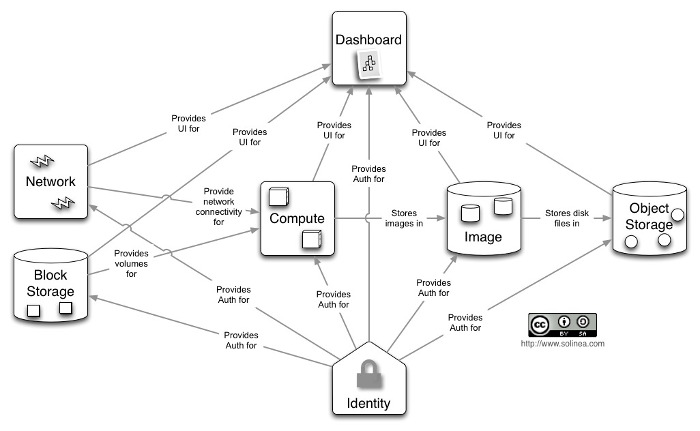
\includegraphics{Images/Openstack_diagramme_conceptuel.jpg}
\caption{Schéma d'organisation des modules d'Openstack \footnotesize{source : http://lea-linux.org/documentations/OpenStack} }
\end{figure}

\subsection{Le client Python nova}\label{le-client-python-nova}

Le client Python-nova est un client en ligne de commande pour le module
Nova OpenStack , il va nous permettre de mettre en oeuvre 100\% de l'API
Nova, et aussi la gestion des instances, des images, etc\ldots{}

\subsubsection{Installation de
python-nova}\label{installation-de-python-nova}

Pour installer le plugin python-nova, il faut avoir préalablement
installé python et son système d'installation pip. Pour lancer
l'installation, il suffit de taper pip install -U python-novaclient .

\subsubsection{Configuration des variables d'environnement pour
Openstack}\label{configuration-des-variables-denvironnement-pour-openstack}

Pour configurer toutes les variables, Openstack génère un fichier RC
contenant la totalité des variables d'environnement à configurer.

Depuis Cloudwatt, il faut aller dans les paramètres \emph{accès et
sécurité} puis \emph{accès API} et enfin télécharger le fichier. En
effet Cloudwatt génère un fichier contenant toutes les variables
d'environnement nécessaire à la configuration de la connexion Openstack.
Ce qui ne sera pas forcément le cas avec un autre service d'hébergement tel qu'Ovh.

L'exécution du fichier se fait grâce à la commande
\texttt{source\ 0750182707\_projet\_tutore\_2017-openrc.sh} et permet la
configuration automatique des variables.

\subsubsection{Liste des instances}\label{liste-des-instances}

La liste des instances créées sont visibles à l'aide de la commande
\texttt{nova\ list}.

\subsection{Création de l'instance}\label{cruxe9ation-de-linstance}

\subsubsection{Génération de la clef
ssh}\label{guxe9nuxe9ration-de-la-clef-ssh}

\texttt{ssh-keygen}
Une clef ssh a été généré pour le porjet, elle ne contient aucune passphrase pour éviter les problèmes de compatibilité avec Ansible. Ce point vas être expliqué plus bas.

\subsubsection{Intégration clef ssh au keypair
Openstack}\label{intuxe9gration-clef-ssh-au-keypair-openstack}

\texttt{nova\ keypair-add\ -\/-pub-key\ .ssh/id\_rsa.pub\ SSHKEY}

\subsubsection{Choix du flavor}\label{choix-du-flavor}

\texttt{nova\ flavor-list} affiche la liste des flavors disponibles. Une
fois choisi, il faut récupérer son ID qui sera renseigné lors de la
création de l'instance.

\subsubsection{Choix de l'image (système
installé)}\label{choix-de-limage-systuxe8me-installuxe9}

\texttt{nova\ image-list} affiche la liste des images systèmes
disponibles. Une fois choisi, Il faut récupérer son ID qui sera demandé
lors de la génération de l'instance.

\subsubsection{Création de l'instance}\label{cruxe9ation-de-linstance-1}

\texttt{nova\ boot\ -\/-key-name\ SSHKEY\ -\/-flavor\ 16\ -\/-image\ 185e1975-c9c5-4358-909e-5e329808902e\ instance1}

Pour la création de l'instance, on retrouve quatre éléments : 
\begin{itemize}
\item le nom du keypair 
\item l'id du flavor 
\item l'id de l'image
\item le nom de l'instance
\end{itemize}
\vspace{5mm}
\begin{figure}
\centering
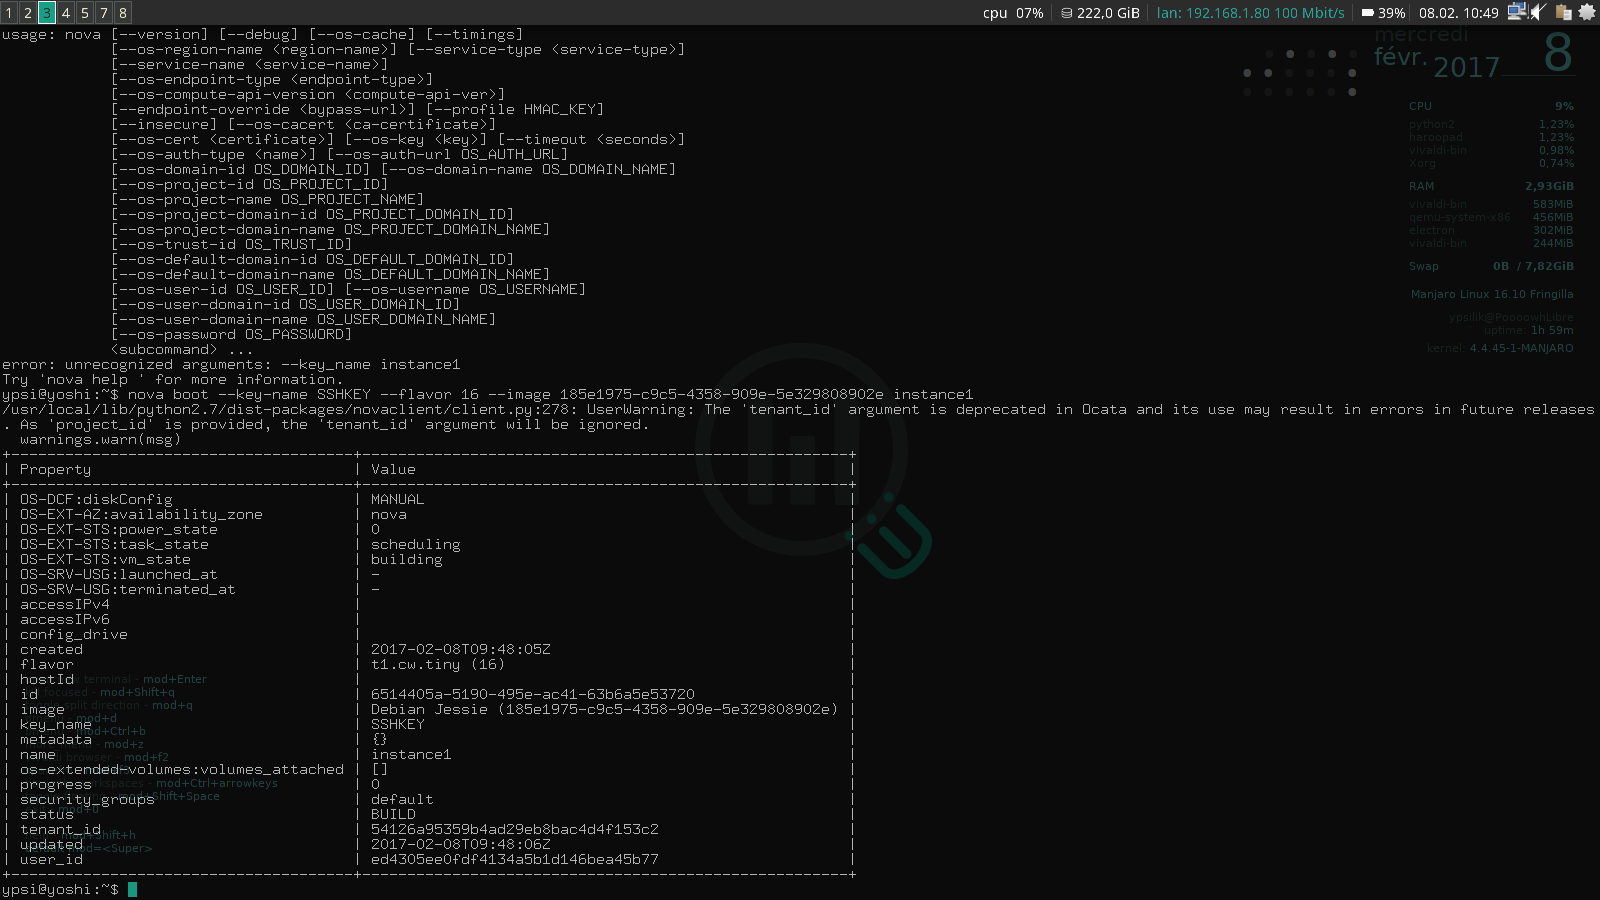
\includegraphics{Images/eeee.png}
\caption{Paramètres demandés par Openstack pour la création d'une instance}
\end{figure}

\newpage
\section{Terraform}\label{terraform}

\subsection{Présentation}\label{pruxe9senation}

Terraform est un outil développé en Go qui permet la gestion
d'infrastructure à l'aide de recettes. L'objectif de ce logiciel est de
permettre une configuration centralisée, rapide et efficace d'une
infrastructure.

Terraform fonctionne avec des fichiers textes pour configurer les futures
infrastructures. Ces fichiers sont appelés \og recette
\fg, ils servent à décrire l'architecture des providers tel
qu'Openstack ou AWS. La configuration se fait dans un fichier
\og main.tf \fg qui est écrit en HCL \footnote{HashiCorp Configuration Language}. La configuration peut aussi être
générée automatiquement par machine avec le format JSON \footnote{JavaScript Object Notation}.
L'extension du fichier sera alors \og main.tf.json
\fg.

Un provider pour Terraform est un service pour le cloud computing, généralement un
IaaS comme c'est la cas pour Openstack. 
Terraform permet de gérer les composants de bas niveau comme les IaaS,
le stockage et la mise à niveau, ainsi que des composants hauts niveaux
comme les entrées DNS et les fonctionnalités SaaS.

Terraform génère un plan d'exécution se basant sur les recettes et
décrivant les étapes qu'il va effectuer. Puis exécute le plan
précédemment défini pour mettre en place l'infrastructure. Terraform
détecte les changements effectués dans les fichiers et créé de nouveaux
plans d'exécution conformément à ces changements.

\subsection{Caractéristiques}\label{caractuxe9ristiques}

\begin{itemize}
\item
  \textbf{Infrastructure as code :} L'infrastructure est décrite en
  utilisant une syntaxe de configuration de haut niveau (HCL). Cela
  permet à une infrastructure d'être versionné et traité comme tout autre
  code.
\item
  \textbf{Plan d'exécution :} Terraform a une étape de \og
  planification \fg qui génère un plan d'exécution. Le
  plan d'exécution montre les actions que Terraform effectuera lorsqu'il
  sera lancé. Cela permet d'augmenter la sécurité en évitant d'avoir des
  surprises lorsque Terraform manipule l'infrastructure.
\item
  \textbf{Graphique des ressources :} Terraform construit un graphique de
  toutes les ressources des infrastructures, et parallélise la création
  et la modification de toutes ces ressources non-dépendantes. Grâce à
  cela, Terraform construit l'infrastructure aussi efficacement que
  possible, et les utilisateurs peuvent avoir un aperçu des dépendances
  de leur infrastructure.
\item
  \textbf{Automatisation des changements :} Des ensembles complexes de
  changements peuvent être appliqués à une infrastructure avec une
  interaction humaine minimale. Pour se faire Terraform se base sur le
  plan d'exécution et le graphique de ressources mentionnés
  précédemment, évitant ainsi des erreurs humaines possibles.
\end{itemize}

\subsection{Quelques cas d'utilisations}\label{quelques-cas-dutilisations}

\subsubsection{Self-service Cluster}\label{self-service-cluster}

Dans de grandes organisations, il devient plus attrayant de créer une
infrastructure \og self-service \fg,
permettant aux équipes de gérer leur propre infrastructure à l'aide de
l'outillage fourni par l'équipe centrale d'exploitation.

A l'aide du fichier de configuration de Terraform on peut rapidement prendre connaissance de l'ensemble de l'infrastructure. Il est alors possible de lancer le script Terraform depuis n'importe quel pc, la seule condition étant d'avoir l'exécutable. Cela représente un réel avantage de portabilité.


\subsubsection{Démos de logiciels}\label{duxe9mos-de-logiciels}

A l'instar de Vagrant qui permet la création d'environnement virtualisé,
les éditeurs de logiciels peuvent fournir une configuration Terraform
pour créer et démarrer une infrastructure de démonstration. Ceci permet
aux utilisateurs finaux de mettre en place rapidement un environnement
de test sur leur propre infrastructure.

\subsubsection{Multi
Cloud-Déploiement}\label{multi-cloud-duxe9ploiement}

Il est souvent attrayant de répendre l'infrastructure sur plusieurs
cloud pour augmenter la tolérance aux pannes. En utilisant une seule
région ou un seul fournisseur cloud, la tolérance aux pannes est
limitée par la disponibilité de ce fournisseur. Avoir un déploiement
multi-cloud permet une meilleure récupération de la perte d'une région
ou tout le fournisseur.

Terraform permet la configuration de plusieurs providers en une seule
configuration. Cela simplifie la gestion et l'orchestration des
providers, en aidant la création d'infrastructures multi-cloud.

\subsection{Syntaxe utilisée}\label{syntaxe-utilisuxe9}

Les configurations de Terraform sont écrites en HashiCorp Configuration
Language (HCL). Ce langage se veut facile à écrire et à lire. L'écriture
des configurations peut aussi se faire en JSON.

\subsubsection{Les bases du langage}\label{les-bases-du-langage}

\emph{Commentaires} - \# sur une seule ligne - /* mon commentaires sur
plusieurs lignes */

\emph{Affectation des valeurs}

\begin{verbatim}
key = value # la valeur peut être une chaîne, un nombre ou un booléen
\end{verbatim}

\emph{Chaînes multilignes} : On utilise
\texttt{\textless{}\textless{}\ -\ EOF} et \texttt{EOF} pour créer des
chaînes multi-lignes ce qui permet principalement d'intégrer des scripts
dans la configuration.

Il existe également de nombreuses fonctions utilisables avec HCL comme
par exemple la fonction format(format, args, \ldots{}) effectuant la mise en forme d'une chaîne de caractère.

Les différents blocs se définissent avec des accolades dans le même
principe que des fonctions dans les autres langages connus.
\texttt{language\ ressource\ "nom\_type\_ressource"\ "nomRessource"\ \{\ \ \ \ \ ...\ \}}

\subsection{Fonctionnement}\label{fonctionnement}

Terraform étant développé en Go, il n'a pas besoin d'être installé. Il
suffit de télécharger une archive .zip et de l'extraire. Il est ensuite
possible d'utiliser les commandes associées à Terraform avec
\texttt{./terraform\ ...}. Pour faciliter l'utilisation des commandes,
il est recommandé de copier le fichier dans \emph{/usr/local/} et
d'ajouter ensuite le chemin menant jusqu'au fichier en question dans le
PATH \texttt{PATH=/usr/local/...:\$PATH}.

\begin{figure}
\centering
\includegraphics{Images/DiagramTerraform2.png}
\caption{Utilisation de Terraform dans un environnement}
\end{figure}

Terraform peut être composé de plusieurs fichiers de configuration pour
une infrastructure. Dans ce cas, les fichiers sont lus par ordre
alphabétique, mais la priorité reste au fichier \emph{main.tf}.

Les fichiers Terraform se composent de différents type de bloc : le bloc
provider et le bloc ressource. Chacun de ses blocs peut se retrouver
plusieurs fois dans un fichier.

\subsubsection{\texorpdfstring{Bloc
\textbf{\texttt{provider}}}{Bloc provider}}\label{bloc-provider}

C'est la partie configuration du provider avec principalement les accès
pour la connexion à celui-ci. Terraform peut contenir plusieurs blocs
provider. Ce bloc gère le cycle de vie des ressources (create, read,
update, delete).
\begin{verbatim}
provider "openstack" {
    user_name  = "admin"
    tenant_name = "admin"
    password  = "pwd"
    auth_url  = "http://myauthurl:5000/v2.0"
}
\end{verbatim}
Cloudwatt offre la génération d'un fichier .sh avec la totalité des
identifiants et accès pour Openstack. Pour la connexion, nous avons pu
omettre le bloc provider, Terraform se charge de récupérer les variables
environnementales correspondant aux paramètres dont il a besoin pour
retrouver le provider.

\subsubsection{\texorpdfstring{Bloc
\textbf{\texttt{resource}}}{Bloc resource}}\label{bloc-resource}

Partie de création et gestion des ressources. Les ressources sont les composants physiques et logiciels qui composent l'infrastructure.

\begin{verbatim}
resource "openstack_compute_instance_v2" "nomTerraform" {
}
\end{verbatim}

\subsubsection{Variables}\label{variables}

Les variables peuvent être externalisées dans un fichier
\og variables.tf \fg ou \og
.tfvars \fg. Pour appliquer des variables enregistrées
sous cette dernière extension, il faut lancer la commande suivante
\texttt{terraform\ apply\ -var-file=variables.tfvars}. Les variables sont
généralement utilisées dans les fichiers .tf sous la forme suivante
\texttt{\$\{var.nomVar\}}.

\subsubsection{Modules}\label{modules}

Il est possible d'intégrer des modules à Terraform. Terraform se charge
du téléchargement et de l'intégration des modules. \\
L'appel d'un module
se fait de la même manière qu'une ressource, mais avec le mot clef
\emph{module}. La source est ensuite indiquée dans une variable. La
source peut provenir d'un dépôt github, d'une archive (de multiples
format sont reconnus comme tar.gz, zip, bz2\ldots{}), d'un dossier
local\ldots{} 

Concrètement un module Teraform est un dossier contenant
des fichiers \emph{.tf} qui ont besoin d'être utilisé plusieurs fois.
Pour régler ce problème de copie multiple du code, il est possible
d'utiliser ce dossier en-tant que module et ainsi avoir un code plus
clair.

Exemple d'un fichier correspondant à un module contenu dans le dossier child.
\begin{verbatim}
variable "memory" {}

output "received" {
  value = "${var.memory}"
}
\end{verbatim}

Appel du module
\begin{verbatim}
module "child" {
  source = "./child"
  memory = "1G"
}
\end{verbatim}


\subsubsection{Plugins}\label{plugins}

Terraform a été crée avec la possibilité d'importer des plugins.
Les plugins servent à rajouter de nouvelles fonctionnalités à Terraform.

Pour installer un plugin, il faut récupérer le code du plugin. Et créer un
fichier \emph{\textasciitilde{}/.terraformrc} contenant un bloc
providers avec une variable indiquant le chemin jusqu'au dossier du
plugin. L'utilisation du plugin se fait après dans le fichier .tf de
l’infrastructure et s'utilise comme un bloc ressource normal en suivant
la syntaxe définie dans la documentation du plugin en question.

\subsubsection{Les commandes}\label{les-commandes}

\begin{itemize}
\tightlist
\item
  \texttt{terraform\ plan} -- génère un plan d'action de la
  configuration. Le plan inclus toutes les actions faites et montre les
  modifications que va effectuer Terraform.
\item
  \texttt{terraform\ plan\ -destroy\ -out=destroy.tf} -- génère un plan
  d'action qui a pour objectif de détruire tous le projet défini pas les
  fichiers de configuration. Le résultat est enregistré dans un fichier
  pour ensuite être appliqué avec \texttt{terraform\ apply\ destroy.tf}.
\item
  \texttt{terraform\ destroy} -- détruit l'infrastructure généré par
  Terraform avec le compte importé (identique à la technique du dessus).
\item
  \texttt{terraform\ apply} -- applique le code Terraform en générant ce
  que \texttt{terraform\ plan} a montré précédemment
\item
  \texttt{terraform\ graph} -- permet la visualisation du plan. Cette
  commande génère un fichier dot qui peut ensuite être transformé en
  image ce qui permet d'obtenir toutes les étapes que va
  effectuer Terraform en schéma.
\item
  \texttt{terraform\ show} -- montre les infrastructures en place
\end{itemize}

\subsection{Configurations
effectuées}\label{configurations-effectuuxe9es}

\subsubsection{Keypair}\label{keypair}

Une des premières configurations effectuées fut l'ajout de clef ssh pour
le projet. Cet ajout avait pour objectif de nous permettre de nous
connecter en ssh avec les instances créées.
\begin{verbatim}
resource "openstack_compute_keypair_v2" "my_keypair" {
  name = "my_keypair"
  public_key = "${var.keypair}"
}
\end{verbatim}
Terraform prend en paramètre pour cette ressource un nom et la clef
publique à ajouter. Cette clef ssh est requise lors de la création
d'instance. En effet, celles-ci prennent en paramètre une keypair -
\texttt{key\_pair\ =\ "\$\{openstack\_compute\_keypair\_v2.my\_keypair.name\}"}
- pour permettre la connexion ssh à l'instance en question. Cependant,
une seule keypair peut être intégrée dans la ressource \emph{instance}.
Pour avoir tous accès en ssh aux instances, nous nous sommes partagés la
clef privé créée spécialement pour le projet et n'ayant pas de
passphrase pour permettre à ansible de se connecter ensuite.

\subsubsection{Instances}\label{instances}

Les instances sont la plus grande partie de la configuration, elles
correspondent aux réseaux privés virtuels (vps) qui vont être créées.
\begin{verbatim}
resource "openstack_compute_instance_v2" "vps" {
  count = 3
  name = "vps-test-${(count.index)+1}"
  image_id = "185e1975-c9c5-4358-909e-5e329808902e"
  flavor_id = "16"
  key_pair = "${openstack_compute_keypair_v2.my_keypair.name}"
  security_groups = ["${openstack_compute_secgroup_v2.terraform.id}"]
  floating_ip = "${element(openstack_compute_floatingip_v2.terraform.*.address,
  count.index+1)}"

  network {
    name = "${openstack_networking_network_v2.network_1.name}"
    fixed_ip_v4 = "192.168.0.1${(count.index)+1}"
  }
}
\end{verbatim}
Une instance peut être créée dans une configuration unique, mais il est aussi possible d'en générer plusieurs automatiquement avec une seule ressource associée grâce au paramètre \texttt{count}.
La création des instances se fait donc en partant de zéro. Avec \texttt{count.index}, nous pouvons récupérer l'index actuel de la boucle générée par Terraform. Chaque instance est rattachée à un ou plusieurs réseaux selon les besoins. Pour notre proof of concept, nous avons utilisé un seul réseau. Pour connecter les instances au réseau, il faut écrire un bloc \textit{network} comme ci-dessus.

\subsubsection{Security group}\label{security-group}

Le security group permet d'autoriser les transmissions sur certain port.
Un security group fonctionne sur le même principe qu'un firewall. Il est
composé de règles \emph{rule}. Une règle est définie pour un port. Nous
avons crées un security group nommé \og terraform
\fg composé d'une seule règle permettant la connexion ssh
(port 22).
\begin{verbatim}
resource "openstack_compute_secgroup_v2" "terraform" {
  name        = "terraform"
  description = "security group"
  rule {
    from_port   = 22
    to_port     = 22
    ip_protocol = "tcp"
    cidr        = "0.0.0.0/0"
  }
}
\end{verbatim}

\subsubsection{Ip flottantes}\label{ip-flottantes}

Les ip flottantes permettent aux instances d'avoir une ip publique, permettant ainsi de pouvoir accéder en ssh aux instances.

Terraform offre la possibilité de générer automatiquement les adresses ip en les
piochant dans un pool public d'adresses. Cependant l'utilisation
d'ansible pour le provisionnement des instances requière la connaissance des adresses ip flottantes attribuées aux machines.

Pour répondre à ce problèmes, plusieurs solutions s'offraient à nous. 
\begin{itemize}
\item La première est l'importation des adresses ip avec
\texttt{terraform\ import}. \\
L'importation avec Terraform fonctionne de la manière
suivante : la ressource est importée avec la commande \texttt{terraform\ import}, et pour être
utilisable, elle doit avoir une ressource créée dans le fichier .tf.
L'importation d'une multitude d'adresses ip entraînent la création du
même nombre de ressources. 
\item La seconde solution est la création d'une liste contenant
les adresses ip flottantes créées depuis l'interface web de l'hébergeur.
L'appel de l'adresse se fait depuis la ressource instance de Terraform
qui vas récupérer une adresse dans la liste.
\end{itemize}

\begin{verbatim}
# Fichier variables.tf
variable "id_ip_flottante" {
    default = ["84.39.49.19","84.39.46.157","84.39.44.165","84.39.41.206"]
}

# Fichier main.tf
resource "openstack_compute_instance_v2" "vps" {
        floating_ip = "${var.id_ip_flottante[(count.index)+1]}"
}
\end{verbatim}

\subsubsection{Réseau, sous-réseau et
routeur}\label{ruxe9seau-sous-ruxe9seau-et-routeur}

Terraform permettant de créer toute une infrastructure, nous nous sommes
aussi penchés sur la création du réseau, de ses sous-réseaux et du
routeur nous permettant un accès au monde extérieur.

\paragraph{Réseau et sous-réseau}\label{ruxe9seau-et-sous-ruxe9seau}

Pour être utilisable, les instances doivent être connectées à un réseau.
Terraform offre la possibilité de créer rapidement et facilement un
réseau ainsi que les sous-réseaux et port utile à celui-ci. Les
instances sont donc configurées pour être intégrées à ce réseau et
obtenir une adresse ip dans ce dernier. 
\begin{verbatim}
resource "openstack_networking_network_v2" "network_1" {
  name = "resTerraform"
  admin_state_up = "true"
}
\end{verbatim}

\subparagraph{Sous-réseau}\label{sous-ruxe9seau}
\begin{verbatim}
resource "openstack_networking_subnet_v2" "subnet_2" {
  name = "SousRes_2"
  network_id = "${openstack_networking_network_v2.network_1.id}"
  cidr = "192.168.0.0/24"
  ip_version = 4 
}
\end{verbatim}

\subparagraph{Port du sous-réseau}\label{port-du-sous-ruxe9seau}
\begin{verbatim}
resource "openstack_networking_port_v2" "port_1" {
  name = "port_1"
  network_id = "${openstack_networking_network_v2.network_1.id}"
  admin_state_up = "true"
}
\end{verbatim}

\paragraph{Routeur}\label{routeur}

Pour que l'infrastructure créée soit opérationnelle, il faut lui
autoriser un accès à l'extérieur du réseau. Pour se faire, nous passons
par un routeur qui est lui-même composé d'une interface le reliant à un
des réseau crée précédemment.
\begin{verbatim}
resource "openstack_networking_router_v2" "router_1" {
  name = "routerTerraform"
  admin_state_up = "true"
  external_gateway = "6ea98324-0f14-49f6-97c0-885d1b8dc517"
}
\end{verbatim}

\vspace{1cm}
Avec la configuration que nous avons effectué tout le long de notre projet, nous sommes arrivés à un environnement fonctionnel et accessible ressemblant à l'image ci-dessous.
\begin{figure}
\centering
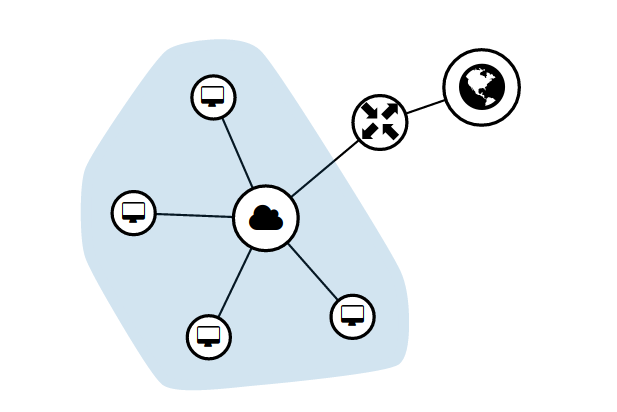
\includegraphics[height=200px]{Images/reseau.png}
\caption{Réseau obtenu avec notre configuration Terraform}
\end{figure}

\newpage
\section{Provisionnement - Ansible}\label{provisionnement}

Terraform permet aussi le provisionnement de ses instances avec
différents provisionners comme Chef, Puppet ou encore Ansible.
Cependant, Terraform n'offre un service que pour Chef.\\
 Mais permet d'exécuter différentes commandes automatiquement depuis la machine
lançant \texttt{terraform\ apply} avec le provisionner
\texttt{local\_exec} ou depuis la machine générée avec Terraform grâce
au provisionner \texttt{remote\_exec}. 

Celui-ci se complète avec le bloc
\texttt{connection} effectuant une connexion ssh avec les identifiants
désiré. Ces dernières se mettant dans les instances. Les ressources de
type \texttt{null-ressource} permettent d'exécuter des commandes après
la création de certaines ressources. Grâce à cela, il est possible de
lancer Ansible automatiquement à la fin de la création des vps.

\subsection{Présentation}\label{pruxe9sentation}

Ansible est un logiciel libre de licence GPL-3.0, crée par Michael
DeHaan et écrit en python. La première version du logiciel date d'avril
2012 et la dernière version est la 2.2.1.0 datant de janvier 2016. \\
Ansible est un outil de gestion de configuration qui se veut plus simple
dans la prise en main que d'autres produits concurrents comme Puppet ou
Chef.

\subsection{Utilisation}\label{utilisation}

D'une manière général, on utilise un outil de gestion de configuration
pour pouvoir maintenir une configuration identique sur différentes
machines que se soit des serveurs ou des machines virtuelles. \\
Il est difficile de pouvoir gérer à la main tout un parc informatique, il est
peu probable que chaque machine aient parfaitement la même configuration
(du par exemple à un oubli) et de plus, la tâche peut être très
répétitive et une réelle perte de temps suivant la taille du parc. Il
est donc conseillé d'utiliser un outil de gestion de configuration qui
va permettre de mettre à jour de façon automatisée des serveurs. \\
Par exemple si on souhaite changer un paramètre ou encore déployer un
nouveau paquet, il nous suffit juste de modifier l'outil de gestion de
configuration. Il permet également de contrôler et de corriger tout
écart dans la configuration.

Pour plusieurs raisons, Ansible est plus simple d'utilisation que les logiciels concurrents. Tout d'abord, il est
agent-less, c'est-à-dire qu'il n'y a pas de configuration de type
client/serveur à gérer. Il faut seulement un serveur ssh sur les
machines à gérer pour qu'elle puisse être configurée par Ansible.

Ansible utilise aussi un langage qui est très simple à aborder, le YAML.
YAML acronyme de Yet Another Markup Language est proposé par Clark Evans
en 2001, il reprend le concepts d'autres langages comme le XML. \\
Le YAMl se veut être le plus lisible possible par tous. Tous les fichiers en
YAML peuvent commencer par --- et terminer par \ldots{} , c'est le
format qui indique le début et la fin d'un document. 
Lorsque l'on fait une liste, chaque élément de la liste est de type \og
key: value \fg que l'on appelle ``hash'' et
``dictionnaire''. Tous les membres d'une liste correspondent à une ligne
qui doivent commencer au même niveau d'indentation et par un tiret plus
un espace. exemple :
\begin{verbatim}
---
# Liste d'OS LInux
OS:
        - Debian
        - Manjaro
        - Linux Mint
        - Ubuntu
...
\end{verbatim}


\subsection{Fonctionnement}\label{fonctionnement-1}

Ansible fonctionne avec des états.
Par exemple :
Pour un dépôt Git, Ansible va déjà vérifier s'il y a déjà eu un git clone, il va alors vérifier que le dossier existe et faire ensuite la mise à jour, dans le cas ou le dossier n'est pas présent il fera le git clone.

Ansible utilise des playbooks pour pouvoir déclarer des configurations,
ce sont la base du système de gestion de configuration et de déploiement
multi-machines. Les playbooks sont écrits en YAML pour ne pas ressembler
à un script de configuration, mais plutôt à un modèle descriptif d'une
configuration. Ces derniers vont donc permettre de décrire les différentes étapes du déploiement.

\begin{figure}
\centering
\includegraphics[height=150px]{Images/ansible_diagramme.png}
\caption{Fonctionnement ansible}
\end{figure}


\paragraph{Les hôtes et les utilisateurs}\label{les-huxf4tes-et-les-utilisateurs}

Tout d'abord quand on crée notre playbook, il va falloir choisir sur
quelles machines on souhaite appliquer le provisionnement. Pour cela, on
utilise un fichier hosts qui va nous permettre de cibler sur quelles
machines on souhaite utiliser le playbook.\\
 Il existe aussi une ligne remote\_user qui permet elle, de choisir le compte utilisateur auquel
on sera connecté sur le host, c'est-à-dire qu'on peut par exemple la
remplir avec root.

\paragraph{La liste des tâches}\label{la-liste-des-tuxe2ches}

Dans chaque playbook, on va trouver une liste de tâches associée à un
hôte. Ces dernières sont exécutées dans l'ordre et une par une. Une
tâche va être identifiée par le champ \textbf{name} qui est affiché lors de
l'exécution, elle doit être lisible et avoir une bonne description pour
permettre de pouvoir l'identifier facilement.
Et on utilise aussi le champ \textbf{state: present} qui va avant d'installer le paquet vérifier si il est déjà présent.

\paragraph{Le premier playbook}\label{le-premier-playbook}

Pour tester le fonctionnement d'Ansible, nous avons tout d'abord essayé
de provisionner une machine virtuelle que nous avions créée précédemment
à l'aide de Terraform. 


On se connecte en ssh sur cette instance avec la commande :

\begin{verbatim}
ssh -i id_rsa_nopass cloud@84.39.46.157
\end{verbatim}

Sur cette machine on va par exemple essayer d'installer des paquets non
présent comme Nginx et Htop. Avec le playbook suivant on va pouvoir
provisionner notre machine virtuelle :

\begin{verbatim}
- hosts: all
  become: true

  tasks:

    - name: Mise à jour 
      apt:
      update_cache: yes

    - name: Installation de Nginx
      apt:
      name: nginx
      state: present

    - name: Installation de Htop
      apt:
      name: htop
      state: present
\end{verbatim}

Ensuite on le lance avec la commande :

\begin{verbatim}
ansible-playbook --private-key=~/.ssh/id_rsa_nopass -u cloud -i 84.39.44.165, 
provisionement.yml
\end{verbatim}

On a :

\begin{figure}
\centering
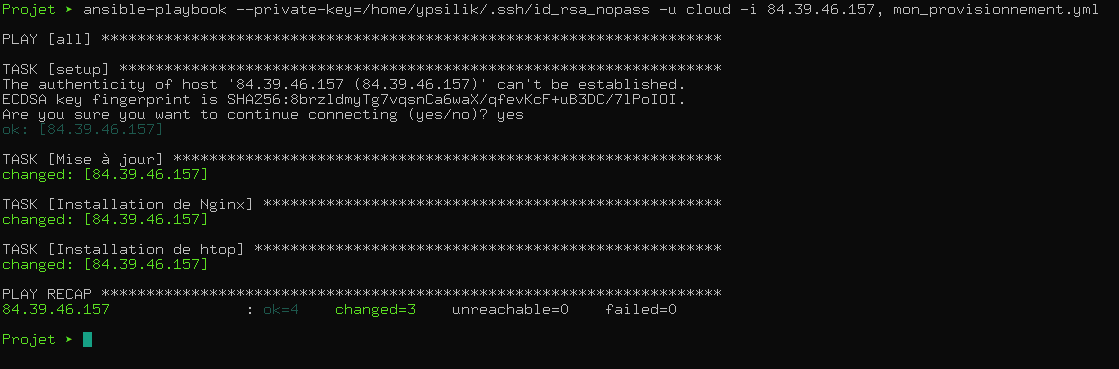
\includegraphics[height=100px]{Images/application.png}
\caption{Exécution ansible}
\end{figure}

Ensuite on peut vérifier la présence de ces derniers en se connectant
sur l'instance :

\begin{figure}
\centering
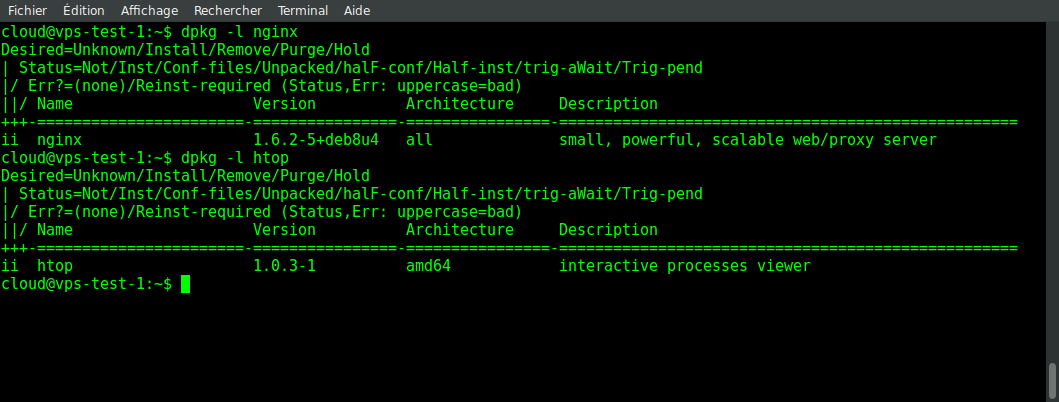
\includegraphics[height=100px]{Images/verification.png}
\caption{Vérification des paquets}
\end{figure}




\subsection{Intégration avec Terraform}\label{intuxe9gration-avec-terraform}

Terraform et Ansible sont deux outils distincts, leurs emplois sont différents.\\
Terraform va permettre de mettre en place l'infrastructure. On va pouvoir décrire la topologie du réseau que l'on souhaite, la taille des instances, ... \\
Ansible, lui, va permettre la configuration de nos instances. Il va définir ce qui se trouve sur les machines, quels logiciels seront présents... C'est un outil de gestion de configuration. Ce n'est pas le cas de Terraform. 

Terraform permet d'utiliser différents outils de gestion de configuration (ansible, puppet ou chef) pour configurer et provisionner les ressources qu'il crée. C'est pour cela que dans notre projet, nous utilisons les deux ensembles, ils ne sont pas en concurrence. 

L'objectif est de pouvoir intégrer Ansible avec Terraform.
C'est-à-dire que depuis notre script .tf on va appeler notre playbook Ansible. 
Comme dit précédemment Terraform permet d'utiliser différents provisionners, mais seul Chef possède un service. 

Pour pouvoir utiliser Ansible, on va utiliser une \textbf{null-ressource}. Les \textit{null-ressource} de Terraform sont des ressources n'étant rattachées à aucune autre ressource, ni aucun type de ressource, ce ne sont donc ni des instances, ni des networks...

La partie \textit{triggers} permet d'attendre la fin de création des instances
\begin{verbatim}
triggers { 
    cluster_instance_ids = "${join(",", openstack_compute_instance_v2.vps.*.id)}"
}
\end{verbatim}

La partie \textit{local-exec} permet de lancer une commande depuis la machine hôte, pour notre projet nous l'avons donc utilisée pour lancer notre commande Ansible.
\begin{verbatim}
command = "ansible-playbook --private-key=~/.ssh/id_rsa_nopass -u 
cloud -i ${element(openstack_compute_instance_v2.vps.*.floating_ip, count.index)},
fichierAnsible.yml"
\end{verbatim}


\subsection{Problèmes rencontrés}\label{probluxe8me-que-lon-a-eu}

Au début avant l'utilisation des null-ressources, nous avions mis l'appel à Ansible toujours dans un provisionner local-exec, mais la position de celui-ci était dans la création du vps. De ce fait, Ansible essayait de se connecter à l'instance avant que celle-ci ne soit complètement créée. \\ Or, Ansible a besoin d'une connexion ssh pour pouvoir fonctionner, et comme les instances
n'étant pas complètement terminées, elles ne pouvaient en aucun cas
assurer une connexion ssh, ce qui provoquait des erreurs.

Pour résoudre ce problème, on a commencé à regarder s'il était possible
qu'Ansible attendent que toutes instances soient créées avant de tenter
une connexion ssh.\\
 Pour cela nous avons utilisé le module
\textbf{wait\_for} d'Ansible qui permet d'attendre une condition
spécifique avant de continuer. Dans notre cas, ce que l'on voulait,
c'était une attente sur le port 22 (port de connexion ssh).

On a donc testé :

\begin{verbatim}
- wait_for :
    port: 22
\end{verbatim}

Mais malgré cette attente, on avait toujours le même problème.

Au fil des tests, on a remarqué que les erreurs venaient le plus souvent
lors de la connexion ssh. Pour éviter tous doutes, nous avons tenté de se
connecter directement à une instance en ssh à  la fin de sa création.
On a vérifié que l'on ne pouvait pas se connecter en
ssh sur nos instances. De fait, nous nous sommes rendu compte que le problème ne
venait peut-être pas de nous, mais de Cloudwatt. 

\newpage
\section{Gestion du projet}\label{ruxe9partition-des-tuxe2ches-au-seins-du-groupe}

Pour pouvoir se partager et aussi pour versionner nos travaux, nous avons utilisé GitHub tout au long de notre projet. \\
Nous avons créé une architecture constituée de 4 dossiers Docs, Notes, Projet et Rapport.\
Dans le dossier Docs, nous avons mis toute la documentation que l'on a pu trouver et qui nous a été utile. Dans le dossier Notes, on peut trouver tout ce que l'on a pu rédiger sur différentes parties de notre projet, à la fois des petits tutoriels, des aides mémoires, ou encore des parties du rapport. Le dossier Projet contient nos différents scripts Terraform et Ansible et pour finir dans Rapport, on peut y trouver le plan de notre rapport, les images utilisées, le rapport final ainsi que nos slides pour le jour de l'oral.

Le projet se tenait sur une seule technologie qui est Terraform. La
répartition des tâches s'est donc faite par rapport aux différentes
parties que nous avons dû créer pour faire fonctionner notre
infrastructure.

\begin{figure}
\centering
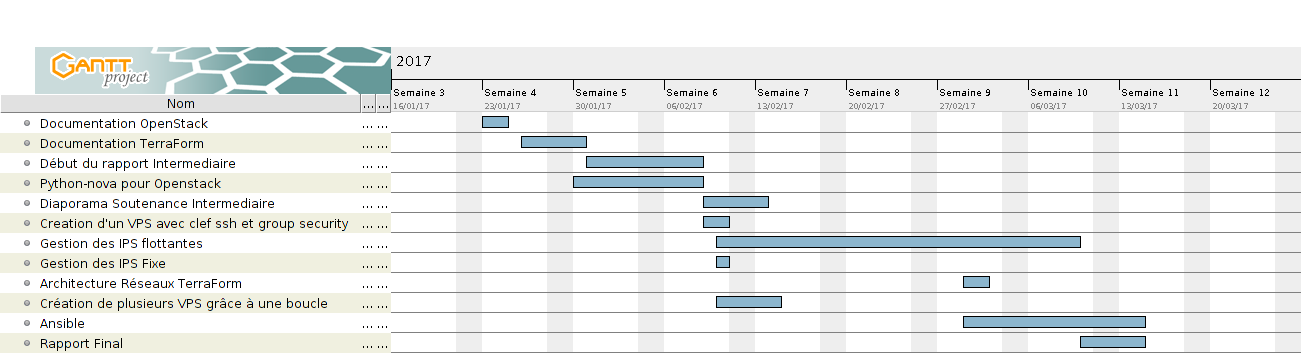
\includegraphics{Images/TerraFormGant.png}
\caption{Diagramme des tâches en fonction du temps}
\end{figure}

\newpage
\section{Avant Terraform}\label{avant-terraform}

\subsection{AWS CloudFormation}\label{aws-cloudformation}

CloudFormation fournit par Amazon Web Service permet de créer et de
gérer un ensemble de ressources qui sont liées, de les ordonner, les
mettre en service et les actualiser. \\
Il permet d'avoir aussi une infrastructure as code avec des simples fichiers textes au
format JSON ou YAML. Il fonctionne uniquement avec AWS, mais le
fonctionnement est semblable à celui de  Terraform. Il permet de créer un modèle qui
décrit toutes les ressources AWS que l'on veut (telles que des instances
Amazon EC2 ou des instances de base de données Amazon RDS). De plus, AWS
CloudFormation s'occupe de leur mise en service et de leur
configuration.\\
AWS CloudFormation propose des modèles d'exemples déjà
créé qui peuvent être utilisés. Il est aussi possible de créer des
modèles personnalisés.

\subsection{Heat}\label{heat}

Heat est un module de la partie orchestration d'OpenStack. La mission du
programme OpenStack Orchestration est de créer un service accessible
pour gérer l'ensemble du cycle de vie des infrastructures et des
applications dans le cloud OpenStack. \\
Heat fournit une orchestration à
base de modèle pour décrire une application cloud. En s'exécutant,
OpenStack appels différentes API pour générer l'exécution d'applications
cloud. Un template Heat décrit l'infrastructure pour une application
cloud dans des fichiers textes qui sont lisibles et modifiables par les
humains, et peut être géré par des outils de contrôle de version. Le
logiciel intègre d'autres composants d'OpenStack. Les modèles permettent
la création de la plupart des types de ressources OpenStack tels que les
instances, ip flottantes, des volumes, des groupes de sécurité, les
utilisateurs, etc. Ainsi que certaines fonctionnalités plus avancées
telles que la haute disponibilité. Heat gère principalement
l'infrastructure, mais les templates intègrent aussi des outils de
gestion de configuration logiciel tels que Puppet et Ansible.

\subsection{Terraform vs les autres
logiciels}\label{terraform-vs-les-autres-logiciels}

Les outils comme CloudFormation, Heat, etc permettent à une
infrastructure d'être codifiée dans un fichier de configuration. Les
fichiers de configuration permettent à l'infrastructure d'être
élastiquement créé, modifiée et détruite. Terraform est inspiré par les
problèmes qu'ils résolvent et élimine complètement les dépendances avec ces services.

Terraform utilise de la même façon des fichiers de configuration pour
détailler la configuration de l'infrastructure, mais il va plus loin par
le diagnostique ainsi que la permission de fournisseurs multiples et des
services combinés et composés. Par exemple, Terraform peut être utilisé
pour orchestrer un AWS et un groupe OpenStack en simultané, en
permettant des fournisseurs du 3ème parti comme CloudFlare et DNSIMPLE
d'être intégré pour fournir des services de DNS et CDN. Ceci permet à
Terraform de représenter et gérer l'infrastructure entière avec ses
services de soutien. Au lieu de seulement le sous-ensemble qui existe
dans un fournisseur seul. Il fournit une syntaxe unifiée, au lieu
d'exiger que des opérateurs utilisent des outils indépendants et
non-interopérables pour chaque plate-forme et service.

Terraform sépare également la phase de planification de la phase
d'exécution, en utilisant le concept d'un plan d'exécution. En exécutant
terraform plan, l'état actuel est actualisé et la configuration est
consulté pour générer un plan d'action. Le plan comprend toutes les
actions à entreprendre. Quelles ressources seront créées, détruites ou
modifiées ? Terraform génère un plan d'exécution décrivant ce qu'il va
faire pour atteindre l'état désiré. En utilisant terraform graph, le
plan peut être visualisé pour montrer les commandes qui vont être
exécutées par celui-ci. Une fois que le plan est capturé, la phase
d'exécution peut être limitée aux seules actions du plan. D'autres
outils combinent les phases de planification et d'exécution, ce qui
signifie que Terraform montre les effets de changement qui va se
produire sur l'infrastructure, qui devient rapidement insoluble dans les
grandes infrastructures. Terraform permet aux opérateurs d'appliquer des
changements avec confiance, car ils savent exactement le résultat qui les attendent.

\subsubsection{Tableau comparatif des solutions}
\resizebox{\textwidth}{!}{
\begin{tabular}{|c|p{4cm}|p{3cm}|l|}
\hline
         & Terraform                                                                & Heat                                   & CloudFormation                  \\ \hline
Plan     & Plan d'exécution des modifications, ajouts et suppressions               & Pas de plan ; exécution directe        & Pas de plan ; exécution directe \\ \hline
Provider & Openstack, AWS, DigitalOcean, Google Cloud, CloudFlare et plein d'autres & OpenStack                              & AWS                             \\ \hline
Graph    & Disponible au format dot \texttt\{terraform graph\}                      & Non                                    & Pas nativement                  \\ \hline
Rollback & Oui, pas automatiquement                                                 & Oui, option à activer dans la commande & Oui par défaut                  \\ \hline
\end{tabular}
}
\newpage
\section{Conclusion}\label{conclusion}

Terraform est un outils formidable permettant de déployer des
infrastructures de manière simple et efficace. Il fournit une syntaxe
simple et unifiée permettant de gérer presque toutes les ressources sans
apprendre de nouveaux outils. En outre, Terraform est un outil open
source. En plus de HashiCorp, la communauté autour de Terraform
contribue à étendre ses fonctionnalités, corriger les bugs et documenter
de nouveaux cas d'utilisation. Terraform aide à résoudre un problème qui
existe dans chaque organisation et fournit un standard qui peut être
adopté pour éviter de réinventer la roue entre et au sein des
organisations.

Terraform permet de représenter tout matériel physique, machine virtuelle, conteneur, courrier électronique, fournisseur DNS. Grâce à cette incroyable flexibilité Terraform permet de résoudre beaucoup de problèmes différents. Il peut gérer une seule application ou il peut très bien gérer un ensemble de centres de données. Dans ce projet, nous avons appris à manier Terraform, il possède encore certaines capacités que nous n'avons pas exploité tel que les modules ou plugins dont nous n'avons pas eu l'utilité pour notre projet.

Ce projet nous a permis d'apprendre à travailler en groupe sur un projet conséquent. Nous avons appris à gérer séparément des tâches tout en mettant en commun nos avancées sur le projet. Nous avons aussi pu voir les difficultés que l'on peut avoir avec un hébergeur cloud comme cloudwatt, notamment l'attente des accès et les quelques problèmes d'accès réseaux que nous avons eu.

\newpage
\section{Bibliographie et Webographie}
\textbf{Terraform}\\
Documentation Terraform : \url{https://www.terraform.io/docs/index.html} \\
Terraform: Up \& Running : \url{http://shop.oreilly.com/product/0636920061939.do } \\
\url{http://www.matt-j.co.uk/2015/03/27/openstack-infrastructure-automation-with-terraform-part-2/}

\textbf{Openstack}\\
Documentation Openstack : Rapport donné en exemple \\
Documentation officielle : \url{http://docs.openstack.org}

\textbf{Ansible}\\
Documentation Ansible : \url{http://docs.ansible.com/ansible/playbooks_intro.html}\\
\url{https://quentin.dufour.io/blog/2015-10-02/ansible}

\newpage
\section{Annexes}
\subsection*{Code Terraform}
\subsubsection*{keypair.tf}
\begin{verbatim}
# Keypair générale
resource "openstack_compute_keypair_v2" "my_keypair" {
  name = "my_keypair"
  public_key = "${var.keypair}"
}
\end{verbatim}

\subsubsection*{network.tf}
\begin{verbatim}
# Réseau
resource "openstack_networking_network_v2" "network_1" {
  name = "resTerraform"
  admin_state_up = "true"
}

# Sous-réseau
resource "openstack_networking_subnet_v2" "subnet_2" {
  name = "SousRes_2"
  network_id = "${openstack_networking_network_v2.network_1.id}"
  cidr = "192.168.0.0/24"
  ip_version = 4 
}

#Port du sous-réseau
resource "openstack_networking_port_v2" "port_1" {
  name = "port_1"
  network_id = "${openstack_networking_network_v2.network_1.id}"
  admin_state_up = "true"
}
\end{verbatim}

\subsubsection*{router.tf}
\begin{verbatim}
# Router
resource "openstack_networking_router_v2" "router_1" {
  name = "routerTerraform"
  admin_state_up = "true"
  external_gateway = "6ea98324-0f14-49f6-97c0-885d1b8dc517"
}

resource "openstack_networking_router_interface_v2" "int_1" {
  router_id = "${openstack_networking_router_v2.router_1.id}"
  subnet_id = "${openstack_networking_subnet_v2.subnet_2.id}"
}
\end{verbatim}

\subsubsection*{securityGroup.tf}
\begin{verbatim}
# Secure group
resource "openstack_compute_secgroup_v2" "terraform" {
  name        = "terraform"
  description = "security group"
  
  rule {
    from_port   = 22
    to_port     = 22
    ip_protocol = "tcp"
    cidr        = "0.0.0.0/0"
  }
}
\end{verbatim}

\subsubsection*{variables.tf}
\begin{verbatim}
# pool
variable "pool" {
    default = "public"
}

# keypair
variable "keypair" {
    default = "ssh-rsa AAAAB3NzaC1yc2EAAAADAQABAAABAQCoj+AJej+p324R08l8Y7trRwe
+2OlmvGHIJNW6U7VWDS0jSFr3QJJQsBIJ1KLCxIP0alveWNqUMz4xbUBof8Ai8ULelN5Gk64EsRmkH2Bncxs
KkoraVYr0hBom+k6d7jyONZLYohtKrGyIRC5h2RfwypCDJkAjV10XpJWOsJCJkPPl
+8vuLNRdyPQqx6iBiy7mwDDuF6oNW7CZK3HPe2n9geZSTtjE18FNvHvCTOITVWSnGdSPy2e89ahemM0B3ROo
aogn76Xw0BeNrhUfywXyA4GaS4F1Y28uduvXIO8QRaIiIWRjhPH83wswjnPnDciPEg7/uAa/yZSy1SXFU5V"
}

#Ip flotantes
variable "id_ip_flottante" { 
    default = ["84.39.49.19","84.39.46.157","84.39.44.165","84.39.41.206"]
} 
\end{verbatim}

\subsubsection*{main.tf}
\begin{verbatim}
# vps 
resource "openstack_compute_instance_v2" "vps" {
  count = 3 
  name = "vps-test-${(count.index)+1}"
  image_id = "185e1975-c9c5-4358-909e-5e329808902e"
  flavor_id = "16"
  key_pair = "${openstack_compute_keypair_v2.my_keypair.name}"
  security_groups = ["${openstack_compute_secgroup_v2.terraform.id}"]
  floating_ip = "${var.id_ip_flottante[(count.index)+1]}" 
  # le +1 c'est parce qu'on a test vps qui utilise le 0

  network {
    name = "${openstack_networking_network_v2.network_1.name}"
    fixed_ip_v4 = "192.168.0.1${(count.index)+1}"
  }
}

resource "openstack_compute_instance_v2" "test-network" {
  name = "test-network"
  image_id = "185e1975-c9c5-4358-909e-5e329808902e"
  flavor_id = "16"
  key_pair = "${openstack_compute_keypair_v2.my_keypair.name}"
  security_groups = ["${openstack_compute_secgroup_v2.terraform.id}"]
  floating_ip = "${var.id_ip_flottante[0]}"
  network {
    name = "${openstack_networking_network_v2.network_1.name}"
    fixed_ip_v4 = "192.168.0.2"
    
  }
}

resource "null_resource" "ansible-provision"{
  triggers { 
    cluster_instance_ids = "${join(é",", openstack_compute_instance_v2.vps.*.id)}"
  }
  count = 3 
  provisioner "local-exec" {
    connection {
        type = "ssh"
        user = "cloud"
       private_key = "${file("/home/ypsilik/.ssh/id_rsa_nopass")}"
    }   
         command = "ansible-playbook --private-key=/home/ypsilik/.ssh/id_rsa_nopass
          -u cloud -i ${element(openstack_compute_instance_v2.vps.*.floating_ip,
           count.index)}, provisionement.yml"
  }
}
\end{verbatim}

\subsection*{Code ansible}
\begin{verbatim}
- hosts: all
  become: true

  tasks:  

    - name: Mise à jour 
      apt:
        update_cache: yes

    - name: Installation de Nginx
      apt:
      name: nginx
      state: present

    - name: Installation de htop
      apt:
      name: htop
      state: present
\end{verbatim}

\end{document}

